
\section{The History of Gamma-ray Astrophysics}
\seclabel{history_gamma_ray_detectors}

% Thorough discussion of all experiments:
%   http://imagine.gsfc.nasa.gov/docs/sats_n_data/gamma_missions.html
%   http://space.about.com/od/telescopesandoptics/a/Gammaray-Astronomy.htm

% Nice history with lots of pictures:
%  http://fermi.gsfc.nasa.gov/science/mtgs/symposia/2012/program/mon/DKniffen.pdf

% Good books with introduction

%  "Very High Energy Gamma Ray Astronomy" by Trevor C. Weekes
%    * seems to have a discussion of the principles of Gamma-ray detection.
%      scintilation detectors, spark chambers.

%  "Cosmic Gamma-Ray Sources" - edited by K.S. Cheng, Gustavo E. Romero

% Very nice reference:
%   http://adsabs.harvard.edu/abs/1984BASI...12..202P

% Nice summary:
%   http://articles.adsabs.harvard.edu/cgi-bin/nph-iarticle_query?1984BASI...12..202P&amp;data_type=PDF_HIGH&amp;whole_paper=YES&amp;type=PRINTER&amp;filetype=.pdf

Astronomy has historically been almost entirely concerned with studying
the photons that arrive from outer space.  Because of their charge
neutrality, photons are not defected by intergalactic electric and
magnetic fields and therefore point back to the objects 
emitting them. Historically, the field of astronomy concerned
the study of visible light.  Slowly, over time, astronomers 
expanded their view across the electromagnetic spectrum.

Infrared radiation from the sun was first observed by
William Herschel in 1980 \citep{herschel_1800_experiments-refrangibility}.
The first extraterrestrial source of radio waves was detected
by Jansky in 1933 \citep{jansky_1933_electrical-disturbances}.

% x-ray: http://en.wikiversity.org/wiki/Radiation_history#cite_ref-Burnight_183-1
The development of rockets and sattelites in the 20th ceuntry allowed
the field of astronomy to expand futher, allowering observations
at wavelengths that would otherwise be absorbed in the atmosphere.
The first ultraviolet observation of the sun was performed in 1946 from a
captured V-2 rocket \citep{baum_1946_ultraviolet-spectrum}.  Observations of
solar x-rays were also first carried out on a captured V-2 Rocket in
1949 \citep{burnight_1949_x-radiation-atmosphere}

It was only natural to wonder about the universe at even higher energies.
As is common in the field of physics, the prediction of
the detection of cosmic $\gamma$-rays far proceded their discovery.
\cite{feenberg_1948_interaction-cosmic-ray} theorized that the interaction
of starlight with cosmic rays could produce $\gamma$-rays through
\ac{IC} upscattering.  Following the discovery of the neutral
pion in 1949, \cite{hayakawa_1952_propagation-cosmic}
predicted that $\gamma$-ray emission could be observed from the
decay of neutral pions when cosmic rays interacted with interstellar
matter.  And in the same year, \cite{hutchinson_1952_possible-relation}
discussed the bremsstrahlung radiation of cosmic-ray electrons.
\cite{morrison_1958_gamma-ray-astronomy} first predicted the detection
of several sources of $\gamma$-rays including solar flares, \acp{PWN},
and active galaxies.

\todo[inline]{
Why Gamma-rays can't make it to the ground
}
    
\todo[inline]{Discuss
Balloon gamma-ray detectors.
See discussion on p859 (comparison with other 
experiments) of Kraushaar et al 1965. 
What was the background from, earth albedo gammas I think?
See also Kraushaar et al 1972 p342's discussion of the balloon
experiments: Hulsizer and Rossi (1949), ... 
See also William Tomkin's section 2.2.1 on 
Balloon experiments (page 8) for references
to galactic plane emission being measured
by balloon experiments in 1970.}


    % Links on Explorer 11
% en.wikipedia.org/wiki/Explorer_11
%http://www.physics.wisc.edu/news/obits/kraushaar_obit.html
% http://heasarc.nasa.gov/docs/heasarc/missions/explorer11.html#reference
% http://articles.adsabs.harvard.edu/cgi-bin/nph-iarticle_query?1965ApJ...141..845K&amp;data_type=PDF_HIGH&amp;whole_paper=YES&amp;type=PRINTER&amp;filetype=.pdf

% "The instrument package weighed 30 pounds, was 20 inches high and 10 inches in diameter. The experimenters believed that they detected 22 cosmic gamma rays."
%  -> http://imagine.gsfc.nasa.gov/docs/sats_n_data/gamma_missions.html
The first space-based $\gamma$-ray detector was \explorerxi
\cite{kraushaar_1965_explorer-experiment}.  It was developed at \ac{MIT}
under the direction of William L. Kraushaar.  It employed a sandwich
scintillator and a Cherenkov counter to direct the position and energy
of incoming $\gamma$-rays and was surounded by a plastic anticoincidence
scintilation counter.  It was launched on boad \explorerxi on April 27,
1961.  The instrument was in opreation for 7 months, but only 141 hours
of data were of acceptable quality.  Using these observations, \explorerxi
observed 31 $\gamma$-rays and, because the distribution a distribution of
these $\gamma$-rays was consistent with being isotropic, the experiment
could not firmly identify the $\gamma$-rays as being cosmic in nature.


% en.wikipedia.org/wiki/OSO_3
% "Their
% next detector, on Orbiting Solar Observatory -3, may be more accurately
% described as having proof of the discovery of cosmic gamma radiation,
% since it found a galactic plane anisotropy of high-energy gammas, much
% later to be confirmed with SAS-2 and COS-B." -- http://imagine.gsfc.nasa.gov/docs/sats_n_data/gamma_missions.html

% Notes: 621 photons, E>100 GeV, 1967, angular resolution +/- 16deg from 
%  ``Cosmic Gamma-Ray Sources`` K.S. Chen, Gustavo E. Romer

\todo[inline]{Describe scintilation detector better.
Read William Tomkin's thesis, page 8. Put a note about how the effective
area was apprximately $9\cm^2$.}

\ac{OSO-3}, also developed by Kraushaar,
followed \explorerxi as the next major astrophysical
$\gamma$-ray detector \cite{kraushaar_1972_high-energy-cosmic}.
The \ac{OSO-3} sattelite 
allowed the on board $\gamma$-ray detected to have
an improved weight, power, telemetry, and expsoure, creating a
more sensitive experiment.

It was launched on March 8, 1967 and operated
for 16 months, measuring
621 cosmic $\gamma$-rays with energies above 50 MeV.
The most important result of the expirment was to
measure a strong anisotrophy in the distribution of 
the $\gamma$-rays with a strong clustering of 
$\gamma$-rays towards the Galactic plane.
\figref{oso3_skymap} shows a skymap of these $\gamma$-rays.
This experiment confirmed both a Galactic component
to the $\gamma$-ray sky as well as an additional isotropic
component, hypothesised to be extragalactic in origin.

\begin{figure}[htb]
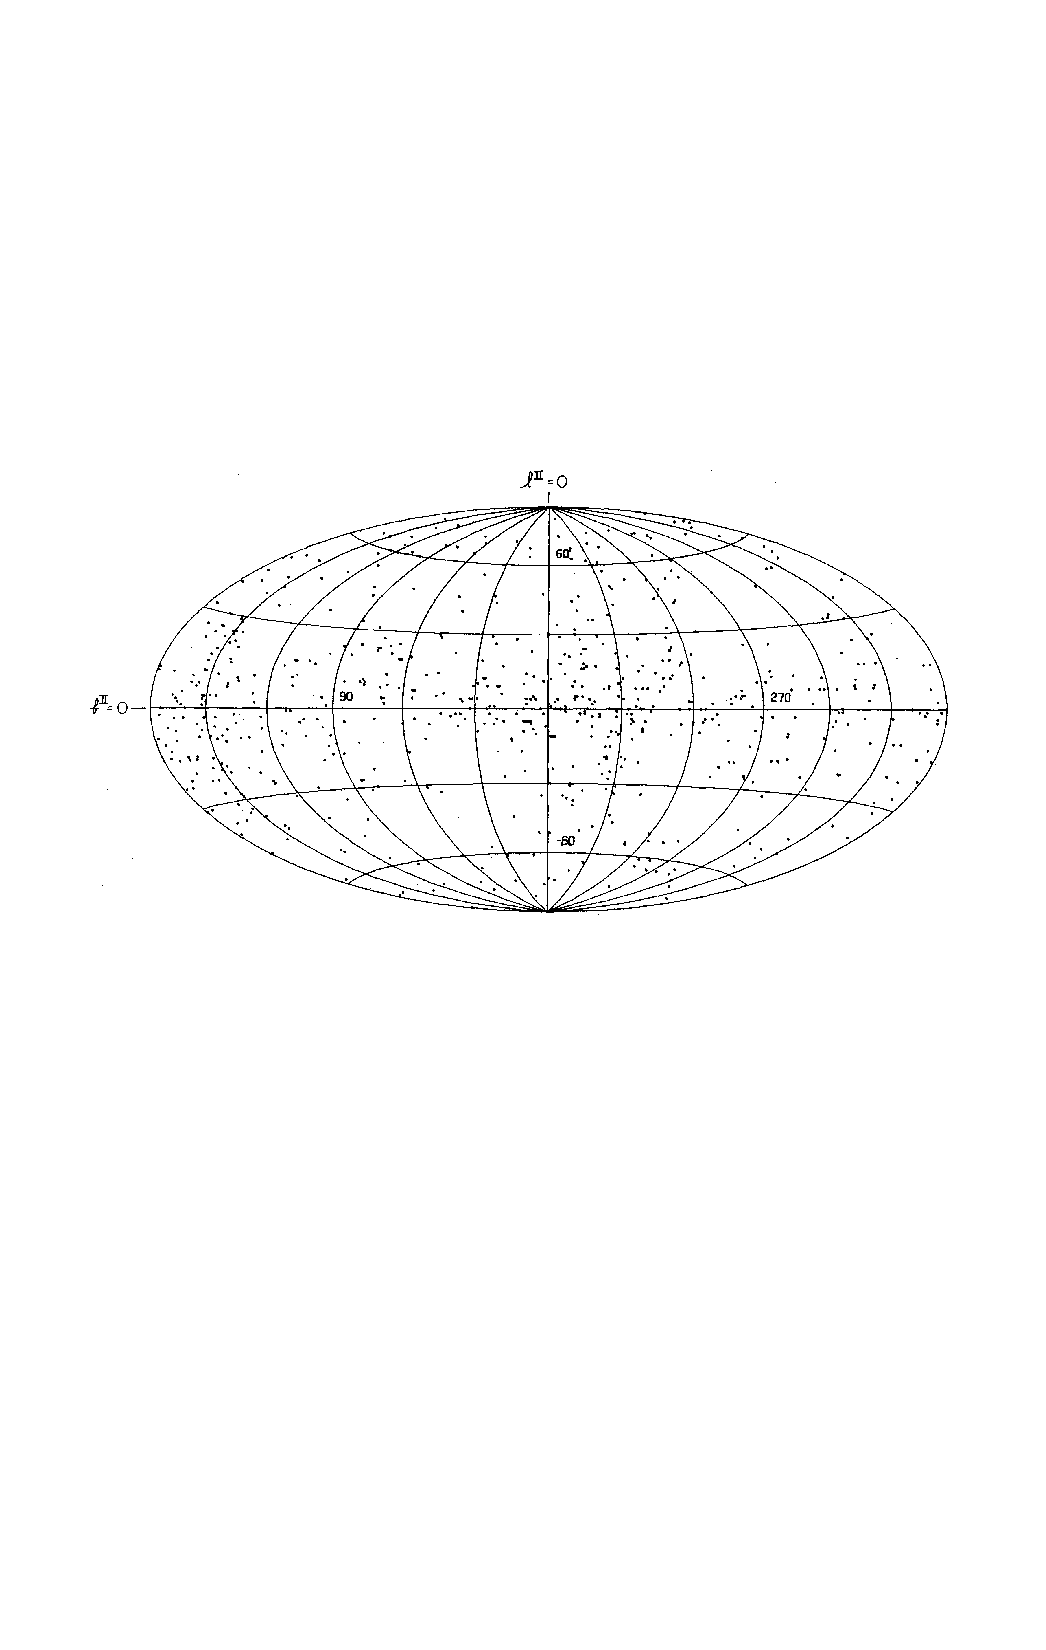
\includegraphics{chapters/introduction/figures/kraushaar_et_al_1972_skymap.pdf}
\figlabel{oso3_skymap}
\caption{The position of all 621 cosmic $\gamma$-rays
detected by \ac{OSO-3}. This figure is from 
\cite{kraushaar_1972_high-energy-cosmic}. }
\end{figure}




\begin{itemize}
\item 

  % ``Additional gamma-ray experiments flew on the OGO, OSO, Vela, and Russian
  % Cosmos series of satellites. However, the first satellite designed as a
  % ``dedicated'' gamma-ray mission was the second Small Astronomy Satellite
  % (SAS-2) in 1972.`` - http://imagine.gsfc.nasa.gov/docs/science/know_l1/history_gamma.html

  \ac{SAS-2}
  

  \item SAS-2
  \item COS-B
  \item EGRET

    % Good summary of EGRET Results:
    %  http://arxiv.org/pdf/0811.0738.pdf
  \item AGILE
\end{itemize}

\subsection{The \fermi Gamma-ray Space Telescope}

\ldots


\subsection{H.E.S.S.}

\ldots
